\documentclass[border=10pt]{standalone}
\usepackage{pgfplots}
\pgfplotsset{compat=1.18}

\begin{document}
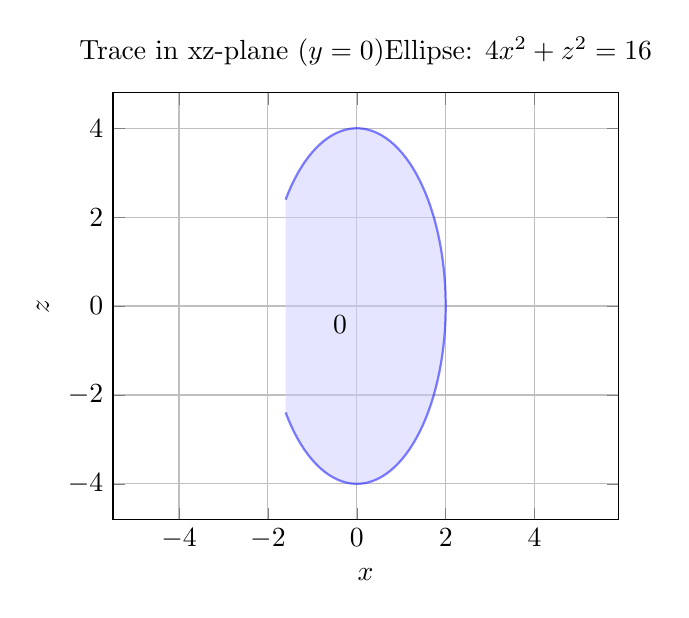
\begin{tikzpicture}
\begin{axis}[
    xlabel=$x$,
    ylabel=$z$,
    title={Trace in xz-plane ($y=0$)\\Ellipse: $4x^2 + z^2 = 16$},
    domain=-2.5:2.5,
    samples=100,
    width=8cm,
    height=7cm,
    axis equal,
    grid=major,
    ]
    % Ellipse: x^2/4 + z^2/16 = 1
    \addplot[blue, thick, fill=blue!20, opacity=0.5] 
        ({2*cos(deg(x))}, {4*sin(deg(x))});
    \addplot[black, thin] (0,0) node[below left] {0};
\end{axis}
\end{tikzpicture}
\end{document}